\documentclass[a4papper, 12pt]{report}

%Csomagok
\usepackage[utf8]{inputenc}
\usepackage[T1]{fontenc}
\usepackage[unicode]{hyperref} %link
\usepackage{amsfonts} %matekos jelölések
\usepackage{amsmath} %matekhoz
\usepackage{graphicx}
\usepackage{algorithx}

\frenchspacing

\title{Második}
\author{Váraljai Péter}
\date{2016.01.01}

\begin{document}
	\maketitle
	\tableofcontents
	\chapter{Első óra}
	%\chapter{Bevezetés}
		\section*{rövid ismertető}
			Ez nincs benne a tartalom jegyzékbe.
		\section{szekció}
			Ez egy fejezet
			\subsection{Alfejezet}
				\paragraph{bekezdés címe}\mbox{} \\ %új sor
				Hello Word!
				
				\noindent %nincs behúzás
				új bekezdés
				
				ez is %van behúzás
		\newpage		
		\section{Felsorolások}
			\subsection{Kötőjelek}
				\begin{description}
					\item[Kicsi:] -
					\item[Nagy:] --
					\item[Gondolatjel:] ---
					\item[Mínusz:] $-$
				\end{description}
			\subsection{itemize}
				\begin{itemize}
					\item felsorolás
					\item ez is\dots
				\end{itemize}
		\section{Betűk}
			\subsection{text\dots}
				\begin{enumerate}
					\item \textbf{vastag}
					\item \textit{dőlt}
					\item \textsf{ezmiez}
					\item \textsc{kiskapitális}
					\item \texttt{írógép}
				\end{enumerate}
			\subsection{egyéb}
			{\tiny pici}
			{\large nagyobb}
			{\Large mégnagyobb}
			{\huge nagyonnagy}
			{\Huge legnagyobb}
	\chapter{Második óra}
	%\section{Matematika}
	$\alpha$
	$a^{1/2}$
	
	\href{http://google.hu}{link}
	
	$_a^bX_c^d$
	
	% & jellhez igazít
	\begin{align}
		lim_{x \rightarrow x_0} \sum_{k=0}^{n} y &\leq f \left( \frac{x}{pi} \right), \quad \forall x \in \mathbb{R}
		\\
		\sum_{k=0}^{n} y &\leq f \left( \frac{x}{pi} \right), \quad \forall x \in \mathbb{R} \nonumber
		\\
		y &\leq f \left( \frac{x}{pi} \right)
		\label{eq:egyenlet1}
	\end{align}
	
	Hivatkozás: \ref{eq:egyenlet1}
	
	\begin{figure}[h!]
		\centering
		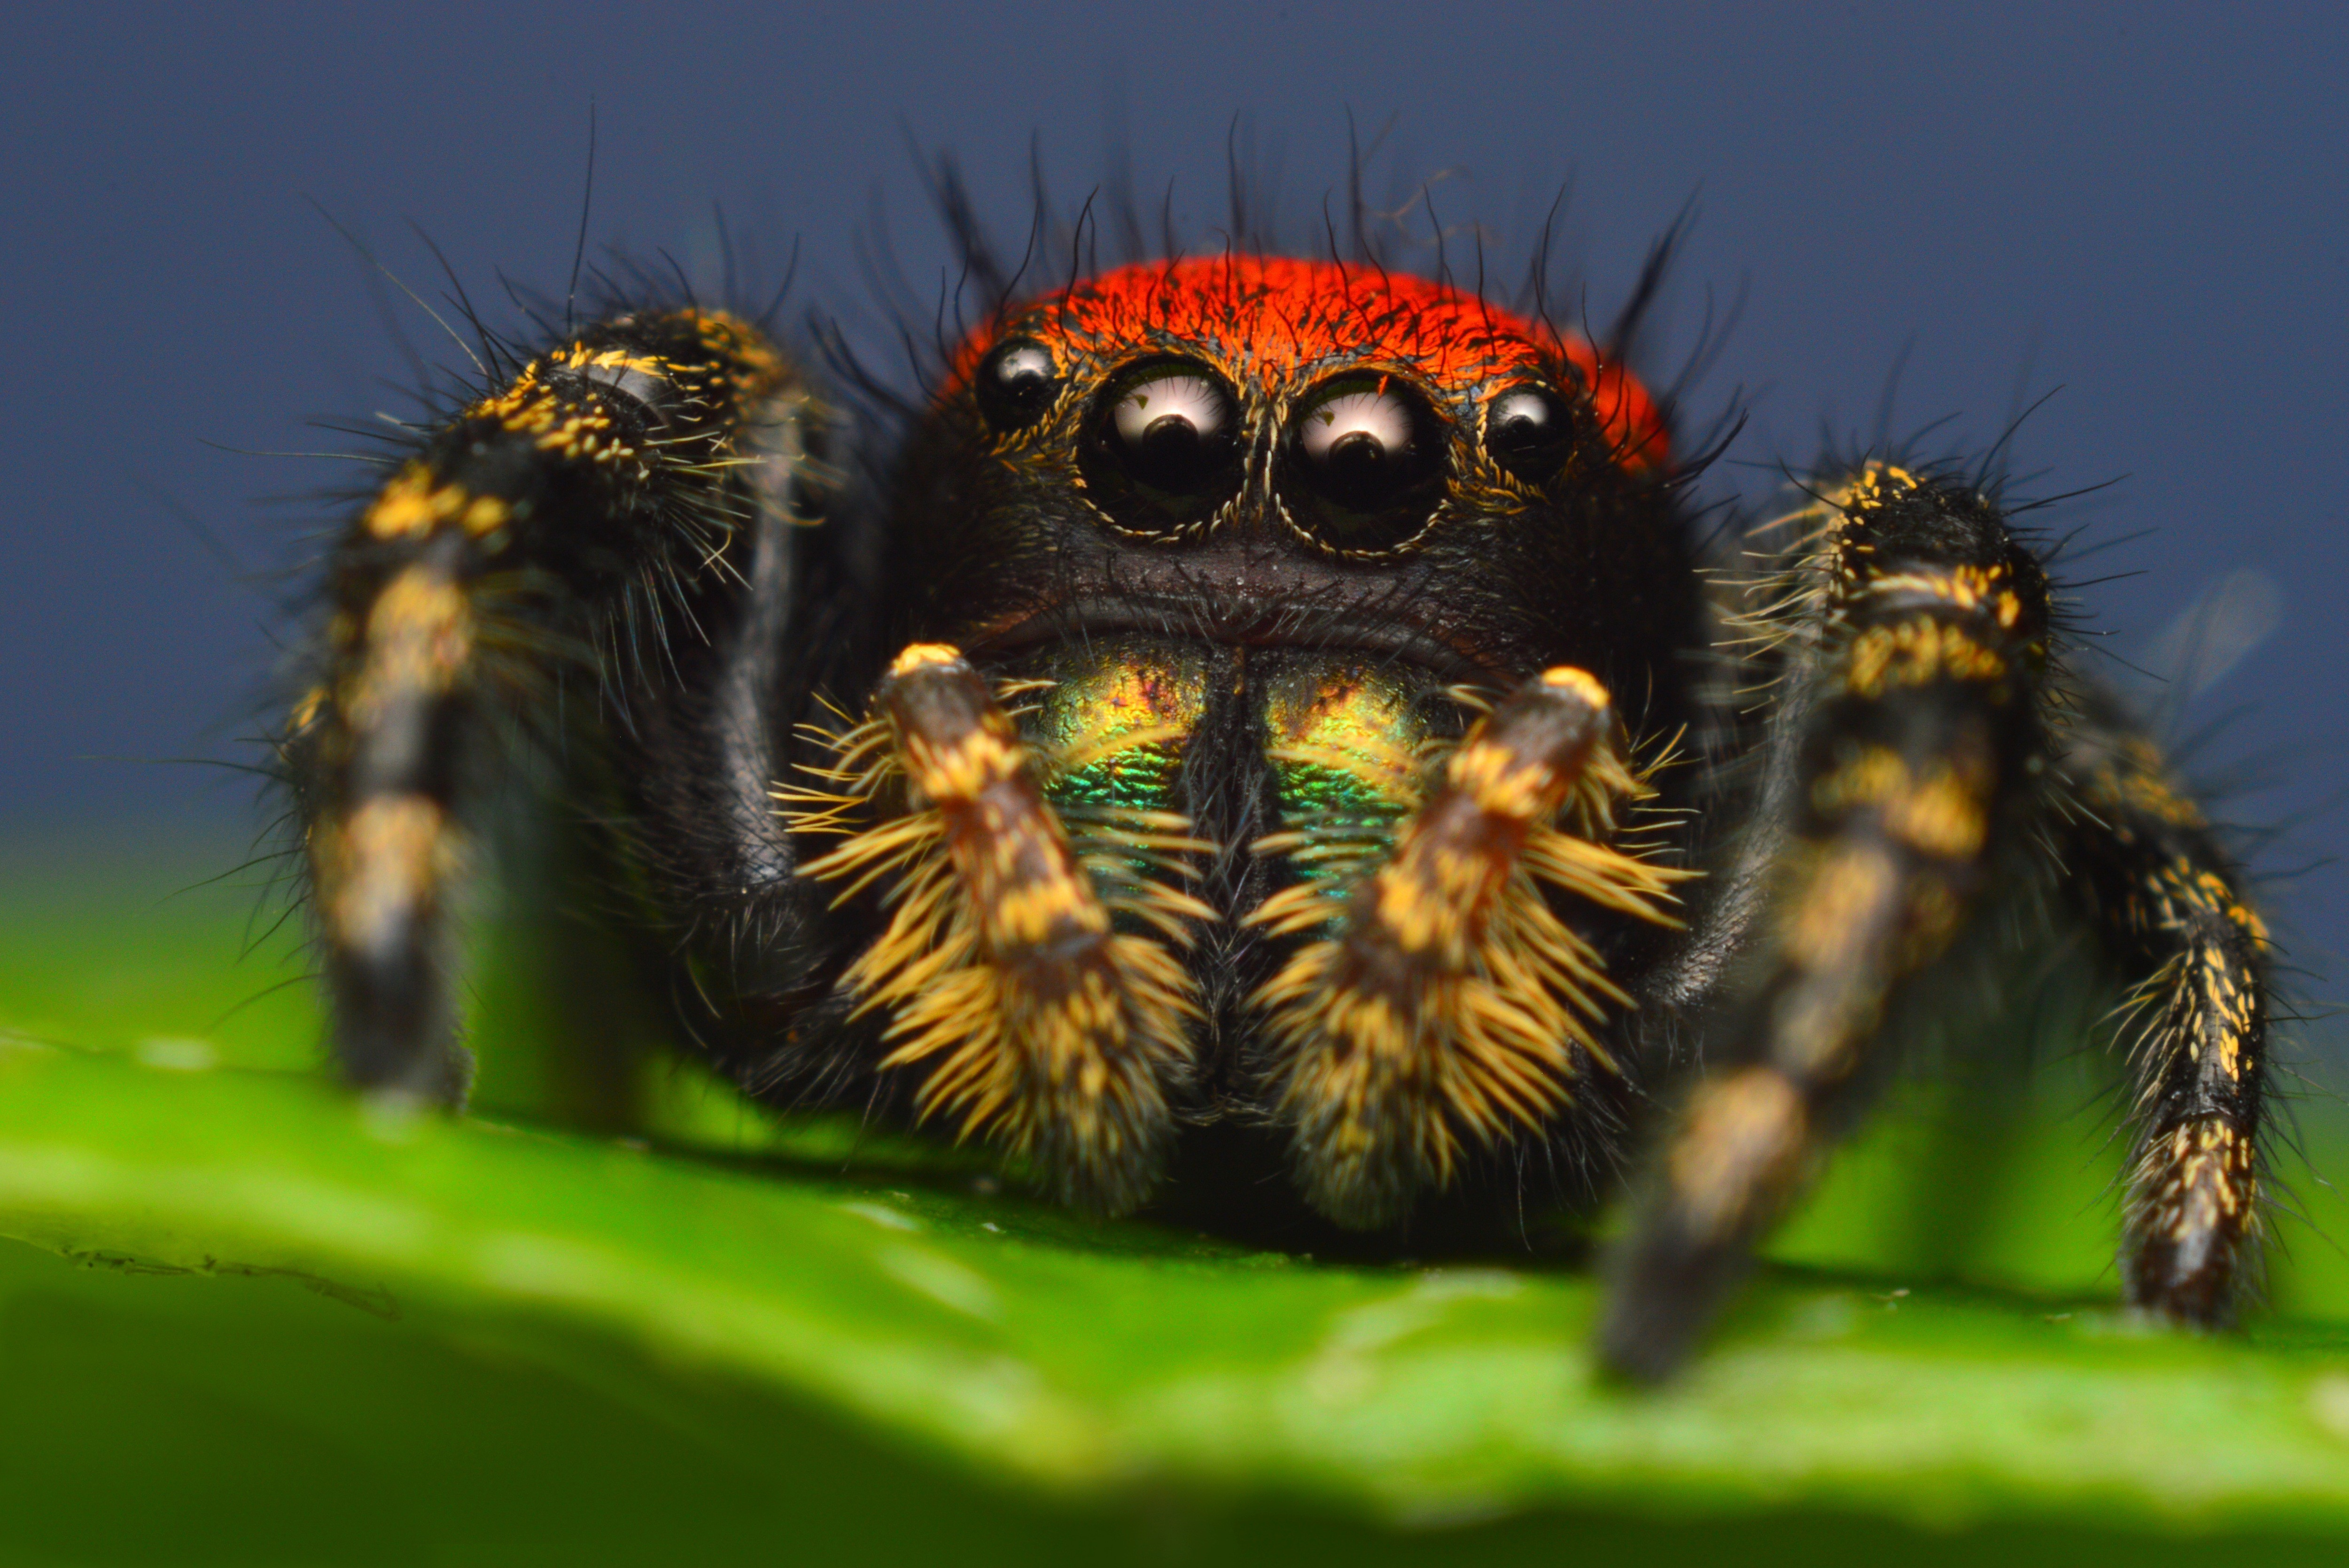
\includegraphics[scale=0.03]{aaa.jpg}
		\label{kep:kep1}
	\end{figure}
	\chapter{3. óra}
	% SECTION: TÁBLÁZATOK    
\section{Táblázatok használata}\label{sec:tablazatok}    

	\begin{table}[!h]
		\begin{center}
        	\begin{tabular}{|l|ccc|}
            \hline
        	Számrendszer  &  Alap &	Jele      & Példa \\
            \hline
			Decimális 	  &  10   &	          & 139  \\
			Bináris 	  &  2 	  & b 	      & 100b \\
			Oktális 	  &  8    & 0 	      & 065 \\
			Hexadecimális &  16   &	0x vagy h & 0x243, 22h\\
            $\pi$-alapú   &  $\pi$ & $\cdots$ & $\cdots$ \\
            \hline
        	\end{tabular}		
		\end{center}
        \label{tab:szamrendszerek}
        \caption[Első táblázat]{A félév elején tanult számrendszerek\dots}
	\end{table}
    
    A babel csomag használatával névelővel is elláthatjuk
    a referenciákat.
    Az utolsó sornál nem kell sortörést jelezni, 
    csak ha vonalat húzunk utána\dots.
    
    Megjegyzés: a táblázat annál szebb, minél kevesebb a vonal
    és ha függőleges nincs, vagy alig észrevehető.
    
    Megjegyzés2: további csomagok segítségével tudunk
    szaggatott vonalat és egyéb vastagságú vonalakat használni.
    
    \subsection{Oszlopok összehúzása}
    	\begin{table}[!h]
		\begin{center}
        	\begin{tabular}{|lccc|}
            \hline
            \multicolumn{4}{|c|}{Közös oszlop}\\
            \hline
        	Számrendszer  &  Alap &	Jele      & Példa \\
            \hline
			Decimális 	  &  10   &	          & 139  \\
			Bináris 	  &  2 	  & b 	      & 100b \\
			Oktális 	  &  8    & 0 	      & 065 \\
			Hexadecimális &  16   &	0x vagy h & 0x243, 22h\\
            $\pi$-alapú   &  $\pi$ & $\cdots$ & $\cdots$ \\
            \hline
        	\end{tabular}		
		\end{center}
	\end{table}
    
\section{Elágazások}

 \begin{equation}	
 f(n) =
  \begin{cases}
    n/2       & \quad \text{ha } n \text{ páros}\\
    -(n+1)/2  & \quad \text{ha } n \text{ páratlan}\\
  \end{cases}
  \end{equation}
  
% SECTION: EGYÉB  
\section{Egyéb tudnivalók} 

	Órai munka: keressetek rá a neten, hogy lehet algoritmust
    közölni latex-ben.
	\footnote{Lábjegyzetet írunk}
    

\section{Idézés}

	Minden tudományos munkában a felhasznált irodalmat idézzünk.
    Soha nem használunk fel irodalmat anélkül, hogy idéznénk.
    Soha.
    Itt egy idézet \cite{nika2016strong}. Ennyi.
    
    Megtudtam, hogy lehet a magyar babel csomagot használni:
    recompile from scratch.
    
    
\bibliographystyle{plain}
\bibliography{bibliography.bib}
	
	\begin{program}
	\mbox{A fast exponentiation procedure:}
	\BEGIN \\ %
  		\FOR i:=1 \TO 10 \STEP 1 \DO
     		|expt|(2,i); \\ |newline|() \OD %
			\rcomment{This text will be set flush to the right margin}
			\WHERE
			\PROC |expt|(x,n) \BODY
          		z:=1;
          		\DO \IF n=0 \THEN \EXIT \FI;
             	\DO \IF |odd|(n) \THEN \EXIT \FI;
				\COMMENT{This is a comment statement};
                n:=n/2; x:=x*x \OD;
            	 \{ n>0 \};
             	n:=n-1; z:=z*x \OD;
         	|print|(z) \ENDPROC
	\END
\end{program}
	
\end{document}